
This chapter gives a concise introduction to the relevant background in Magnetic Resonance Fingerprinting and its current applications. 
It begins with an overview of existing quantitative MR techniques with a particular emphasis on $T_1$ and $T_2$ relaxation times and introduces the general MRF framework.
%along with some of its current applications.

\hfill

% % % % % % % % % % % % % % % % 
\section{Quantitative MRI}\label{chapterlabel2sec21}
Quantitative Imaging is an image acquisition and processing technique whose main objective is to attach a scientific-grade measurement to every pixel in the image such that it can be interpreted independently of the scanner, session, or patient. 
In the medical sciences, quantitative imaging has always been a long-standing goal as it can potentially provide less variability in interpretation, and a higher level of objective evaluation.
However, not all medical imaging techniques are quantitative. 
Conventional MRI, for example, relies on the acquisition of `weighted images', where the image contrast is dependent on both the experiment specifics and tissue properties. 

\hfill

Quantitative Magnetic Resonance Imaging aims to overcome these limitations by providing specific measures of the underlying tissue properties. 
These can include a wide variety of measures such as the proton density of tissue, metabolite concentrations, macromolecular proton fractions, diffusion of water molecules, and others.
However, a large body of research is dedicated to quantifying the $T_1$ and $T_2$ relaxation times of the underlying tissue. 
These metrics have raised a significant interest in the MR community as it was observed that $T_1$ and $T_2$ measures can identify cancerous cells \cite{Damadian1151}, iron accumulation in patients with Parkinson's Disease \cite{JosefVymazal1999}, and inflammation or neural tissue degeneration in multiple sclerosis \cite{MillerD1998}.

\hfill

One drawback of quantitative MRI is that it has a lengthier scan time than conventional MRI. 
For example, $T_1$ and $T_2$ mapping relies on acquiring several images, each with all sequence parameters kept fixed and one specific parameter varied from one acquisition to the next. 
These images are then fitted with a mathematical model in order to estimate the parameters of interest, such as the longitudinal relaxation time $T_1$ \cite{LookLocker1970} or the transverse relaxation time $T_2$ \cite{Giri2009}. 
More recently, other approaches have shortened the acquisition time \cite{Doneva2010} or have provided concurrent measurements of both $T_1$ and $T_2$ \cite{Schmitt2004} relaxation times.
However, these techniques are limited in the number of properties they can retrieve and the accuracy of quantification.

\hfill

To overcome these limitations, a novel quantitative imaging technique called Magnetic Resonance Fingerprinting was developed.
The following section will provide an overview of the MR fingerprinting framework, together with some of its current applications and limitations.

\hfill

% % % % % % % % % % % % % % % % 
\section{The MRF framework}\label{chapterlabel2sec22}

Magnetic resonance fingerprinting (MRF) is a novel quantitative MR imaging method that provides simultaneous measurements of multiple tissue properties in a single acquisition \cite{Ma2013}. 
This technique has recently sparked the interest of many MR scientists and radiologists because it has the potential to detect and analyze early tissue changes, thus improving the information for diagnosis and research in both clinical and preclinical environments. 

\hfill

MRF takes a different approach on performing quantitative MRI than conventional techniques. 
It relies on the assumption that there is a way to construct an MR sequence such that every type of tissue can give rise to unique signal profiles, much like the way our human fingerprints can uniquely identify a person.
In their paper, Ma et al showed that by varying the acquisition parameters in a pseudorandom fashion, the signal can be kept in its transient state.
Moreover, its temporal shape will be different depending on the underlying tissue properties \cite{Ma2013}.

\hfill

\large \textbf{Acquisition Protocol} \normalsize

Every Magnetic Resonance Fingerprinting solution starts with designing the acquisition protocol.
In the original implementation, Ma et al. designed the pulse sequence starting from an inversion recovery balanced steady state free precession (IR-bSSFP) sequence \cite{Ma2013}.
Their decision was based on the knowledge that this type of sequence is known to be sensitive to $T_1$, $T_2$ and off-resonance frequencies \cite{Schmitt2006}.
More recently, a FISP-type sequence was successfully used by Jiang et al. which removes the banding artifacts caused by the bSSFP sequences \cite{Jiang2015}. 
This has now become the most popular form of MRF for $T_1$ and $T_2$ quantification.

\hfill

However, the MRF framework is highly versatile.
The literature to date shows that for different parameters of interest, the pipeline can be adapted to incorporate ideas from other MR sequences.
For example, Jiang et al. \cite{Jiang2017} showed promising results in generating apparent diffusion coefficient (ADC) maps on top of $T_1$ and $T_2$ maps, by incorporating diffusion-preparation modules \cite{Thomas1998} in a FISP-based MRF sequence.
For brain hemodynamics, Su et al. \cite{Su2017} introduced Arterial Spin Labelling (ASL) `label' and `control' modules in the pipeline and created cerebral blood flow (CBF) and bolus arrival time (BAT) maps.
Finally, for cardiac MRI, data was collected only during diastole in a study held by Hamilton et al. \cite{Hamilton2017} and single slice $T_1$ and $T_2$ maps in the heart were generated.

\hfill

After the sequence protocol has been selected, the MRF framework becomes a three stage pipeline which is summarised in Figure~\ref{fig:mrfPipeline} and in the following sections.

% % % % % % % % % % % % % % % % % % % % % % % % 
\hfill

\large\textbf{Data collection} \normalsize

In the data collection step, two types of datasets are constructed.
\begin{itemize}
    % % % % % 
    \item \textbf{Dictionary.} First, signal evolutions are generated for a wide range of tissue properties and then stored in a database called dictionary. 
    For bSSFP-type sequences, Bloch based
    %or Bloch-McConnell 
    simulations are used to generate the signals \cite{Hamilton2015}.
    For FISP-type sequences, where dephasing across a voxel has to be taken into account, a more sophisticated algorithm is used, called the `extended phase graph' formalism \cite{Weigel2015}. 
    
    In terms of tissue properties, most studies consider the $T_1$ and $T_2$ relaxation times \cite{Ma2013} \cite{Jiang2015} \cite{Hamilton2017} \cite{Gao2015} \cite{Amthor2017} \cite{Buonincontri2017}.
    Other applications are interested in more sophisticated properties such as the apparent diffusion coefficient \cite{Jiang2017} or cerebral blood volume, mean vessel radius and oxygenation maps \cite{Christen2014}.
    
    Finally, a few studies have introduced system parameters.
    Cloos et al. \cite{Cloos2016} investigated the usage of multi-transmit coils in an MRF application for titanium hip implants.
    The study introduced alternating $B_1^+$ illumination profiles interwoven in the MRF sequence and coined it as plug-and-play MRF (PnP-MRF), while successfully quantifying the $B_1^+$ non-uniformities together with the desired tissue properties.
    However, this technique requires multi-transmit RF coils with different illumination profiles that are not yet available in every centre.
    For this reason, Buonincontri et al. \cite{Buonincontri2017} introduced abrupt changes in flip angles in the MRF acquisition sequence to estimate the $B_1$ field without using special equipment.
    
    % % % % % 
    \item \textbf{Images.} After the desired application-dependent dictionary has been created, the image acquisition step is performed using the same sequence parameters as in the dictionary creation stage.
    In the original MRF implementation, Ma et al. \cite{Ma2013} used a variable density spiral acquisition which was rotated from one $T_R$ to the next.
    To fully sample k-space, they acquired the same dataset 48 times, each time with a different starting angle of the spiral.
    Although spiral acquisitions are popular among MRF applications, other techniques have also been investigated.
    For example, Cohen et al. \cite{Cohen2016} used fully sampled Cartesian EPI acquisitions, while Cloos et al. \cite{Cloos2016} used radial acquisitions.

\end{itemize}

% % % % % % % % % % % % % % % % % % % % % % % % 
\hfill

\large \textbf{Pattern recognition} \normalsize

After the acquisition, a pattern recognition algorithm is used to retrieve the parameters of interest.
In the original MRF implementations, a vector dot-product was performed between every acquired signal and the dictionary \cite{Ma2013} \cite{Jiang2015}. 
The dictionary signal that gave the highest score was then chosen to be the most representative one for the voxel that was under investigation.
However, this technique can be time consuming for very large dictionaries.
For this reason, more recent studies have looked into ways of speeding up the process.
For example, McGivney et al. \cite{McGivney2014} used SVD compression to reduce the size of the dictionary.
This led to a speed up in the pattern matching step.
Cauley et al. \cite{Cauley2015fgm} divided the dictionary into several groups based on correlations between entry points and performed the matching only on a representative signal of a group, thus finding the best match more quickly.


% % % % % % % % % % % % % % % % % % % % % % % % 
\hfill

\large \textbf{Information retrieval} \normalsize

The final step of the pipeline is the information retrieval step.
This step involves the creation of the quantitative maps.
This is done by repeating the pattern matching process for every voxel in the acquired images and retrieving the tissue parameters that were used to generate the most representative dictionary signal.
This can also be seen in part three of Figure~\ref{fig:mrfPipeline}.

\hfill

Good quality maps require a number of conditions to be achieved.
First, a large enough dictionary must be created to account for a wide range of possible tissue parameter combinations.
Second, for pseudo-random acquisition parameters, a long enough sequence is needed to allow for better discrimination between signals coming from different tissues. 
More recently, Zhao et al. \cite{Zhao2017}, Cohen et al. \cite{Cohen2016} and Sommer et al. \cite{Sommer2017} investigated ways to optimise the sequence for both better encoding capabilities and shorter scan time.
Finally, high quality maps require that the sample does not move.

\hfill

\textbf{Motion.} The motion robustness of this technique has been investigated in the original MRF implementation by Ma et al. \cite{Ma2013} where the volunteer was asked to randomly move his/her head during the last 3s of a 15s scan.
In this case, the authors reported that the final maps were not affected by the movements.
However, a more recent experimental study conducted by Yu et al. \cite{Yu2017} investigated various types of motion occurring at different times during the scan.
Using radial acquisition, their results show that $T_1$ maps become blurry if the motion happens early in the scan, while $T_2$ maps are mostly affected when motion happens in the middle.
However, in experimental studies it is hard to quantify the type and amount of motion the volunteer has performed.
Therefore, one of the aims of my work is to investigate the impact of motion in an MRF experiment in a controlled and reliable manner, which can only be achieved through simulation.

\begin{figure}[ht]
    \centering
    % \makebox[\textwidth][c]{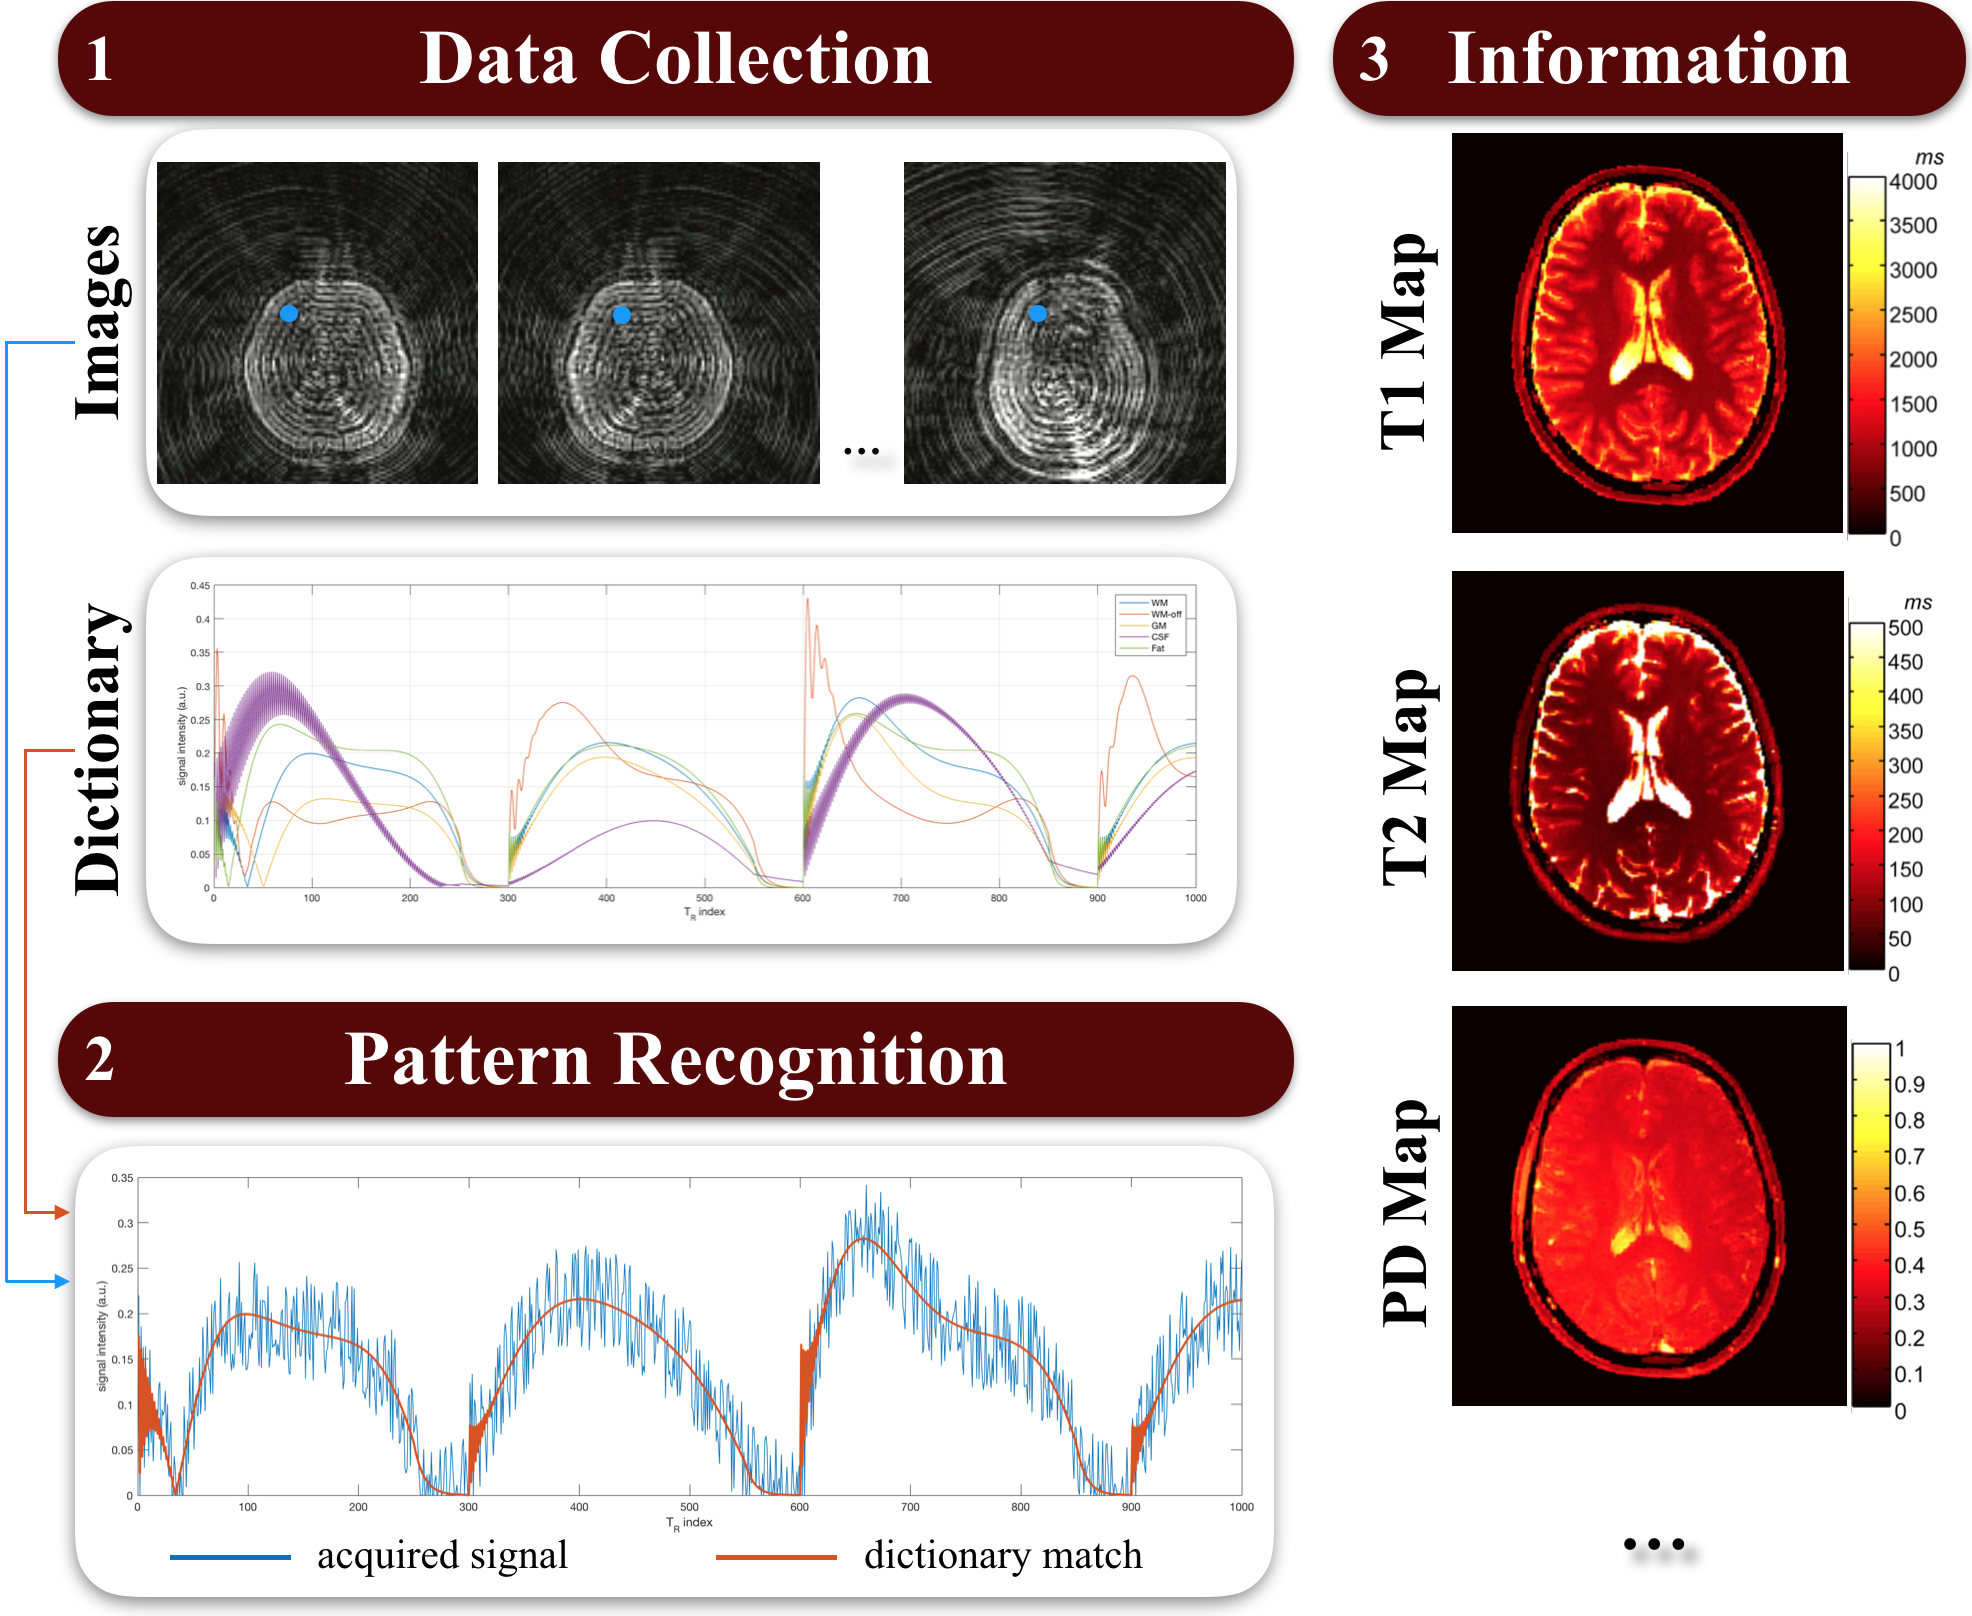
\includegraphics[width=1.4\textwidth]{images/mri/mrfPipeline}}%
    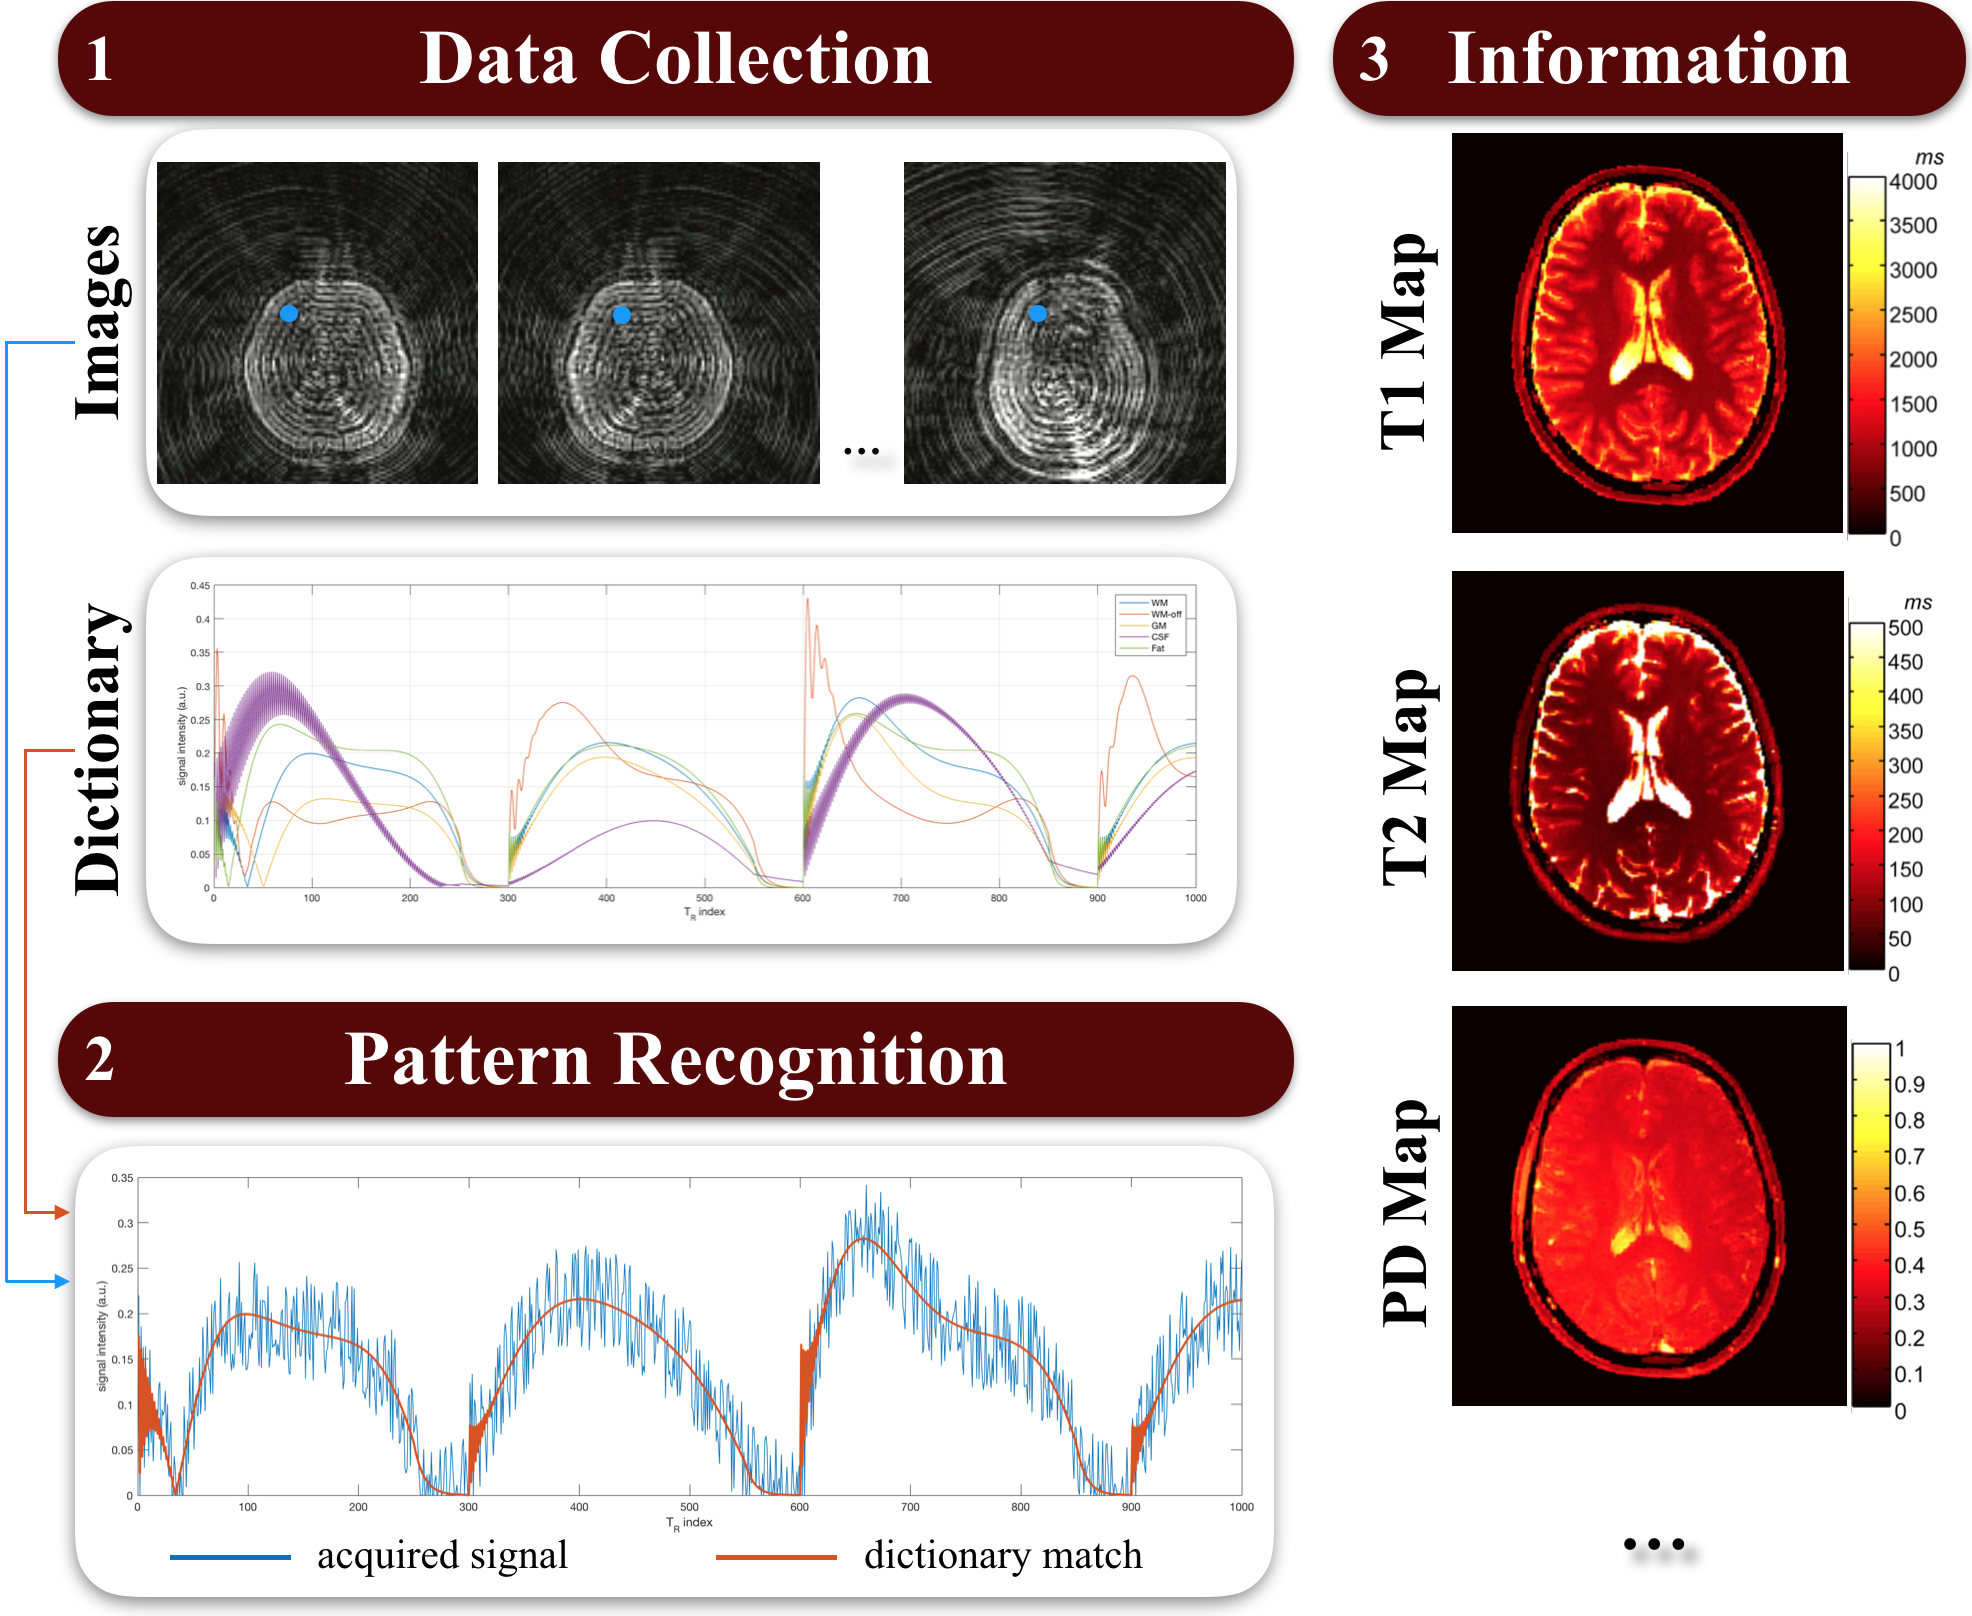
\includegraphics[width=1\textwidth]{images/mri/mrfPipeline}
    \caption{The MRF pipeline: \textbf{(1)} in the first stage images are collected and the dictionary of signals is simulated; \textbf{(2)} in the second stage the pattern recognition algorithm is performed between every acquired signal and the dictionary; the dictionary signal with the highest score is then chosen as the most representative one for that voxel; \textbf{(3)} in the final stage the information associated with each match is retrieved and the quantitative maps are created}
    \label{fig:mrfPipeline}
\end{figure}

